%====================================================================================
\section[Consumo]{Externalidades de consumo}
%====================================================================================

\begin{frame}{Externalidades de consumo}
Consideremos una economía con dos consumidores $(h=1,2)$ y dos bienes $(x,z)$. Los consumidores tienen las funciones de utilidad:
	$$U^1 = x^1 + u_1(z^1) + v_1(z^2) \qquad U^2 = x^2 + u_2(z^2) + v_2(z^1)$$
\medskip
La oferta del bien $x$ proviene de las dotaciones individuales.\medskip

La externalidad surge por el consumo del bien $z$. El bien $z$ es producido en un mercado competitivo que utiliza una unidad de $x$ para producir una unidad de $z$.
Para simplificar: $p_x=1, p_z=1$.
\end{frame}
%------------------------------------------------
\begin{frame}{Externalidades de consumo}
El equilibrio competitivo es descrito por:
	\begin{gather*}
		u_{h}^{\prime}\left( z^h\right) = 1 \quad , \quad h = 1, 2\\
		x^h +z^h = w ^h \quad , \quad h = 1, 2\\
		x^1 + z^1 + x^2 + z^2 = w^1 + w^2
	\end{gather*}
Para cada consumidor el beneficio marginal privado de cada bien, determinado por la utilidad marginal, es igualado con el costo marginal privado. La externalidad no aparece directamente en la determinación del equilibrio.
\end{frame}
%------------------------------------------------
\begin{frame}{Externalidades de consumo}
Las asignaciones Pareto eficientes son halladas resolviendo:
		\begin{align*}
			& \text{Max } \quad U^1 + U^2 = \left[ x^1 + u_1\left(z^1 \right) + v_1\left(z^2 \right) \right] + \left[ x^2 + u_2\left(z^2 \right) + v_2\left(z^1 \right) \right]\\
			& \begin{array}{ll}
				\text{s.a: } & w^1 + w^2 - x^1 - z^1 - x^2 - z^2 \geq 0
			\end{array}
		\end{align*}
La solución es caracterizada por:
	\begin{gather*}
		u_1\left(z^1 \right) + v_1\left(z^2 \right) = 1\\
		u_2\left(z^2 \right) + v_2\left(z^1 \right) = 1
	\end{gather*}
La externalidad conduce a una divergencia entre la valoración privada $(u_{h}^{\prime})$ y la social $(u_{h}^{\prime} + v_{\tilde{h}}^{\prime})$.
\end{frame}
%------------------------------------------------
\begin{frame}{Externalidades de consumo}
	\begin{itemize}
		\item Si la externalidad es positiva $v_{h}^{\prime} > 0$
				\begin{itemize}
					\item La utilidad marginal de cada consumidor es menor en la asignación eficiente que en el equilibrio de mercado
					\item Se consume poca cantidad de z en equilibrio
				\end{itemize}
		\item Si la externalidad es negativa $v_{h}^{\prime} < 0$
				\begin{itemize}
					\item La utilidad marginal de cada consumidor es mayor en la asignación de eficiencia que en el equilibrio de mercado
					\item Se consume demasiada cantidad del bien z en equilibrio.
				\end{itemize}
	\end{itemize}
\end{frame}
%------------------------------------------------
\begin{frame}{Externalidades de consumo}
	\begin{multicols}{2}
		\begin{itemize}
			\item En el resultado de mercado se iguala el beneficio privado marginal $(BPM)$ al costo marginal $(CMg)$
			\item En la asignación óptima se iguala el beneficio social marginal $(BSM)$ al $CMg$
			\item La posición del $BSM$ respecto al $BPM$ depende del efecto externo.
		\end{itemize}
		
		\begin{center}
			\vspace{-0.5cm}
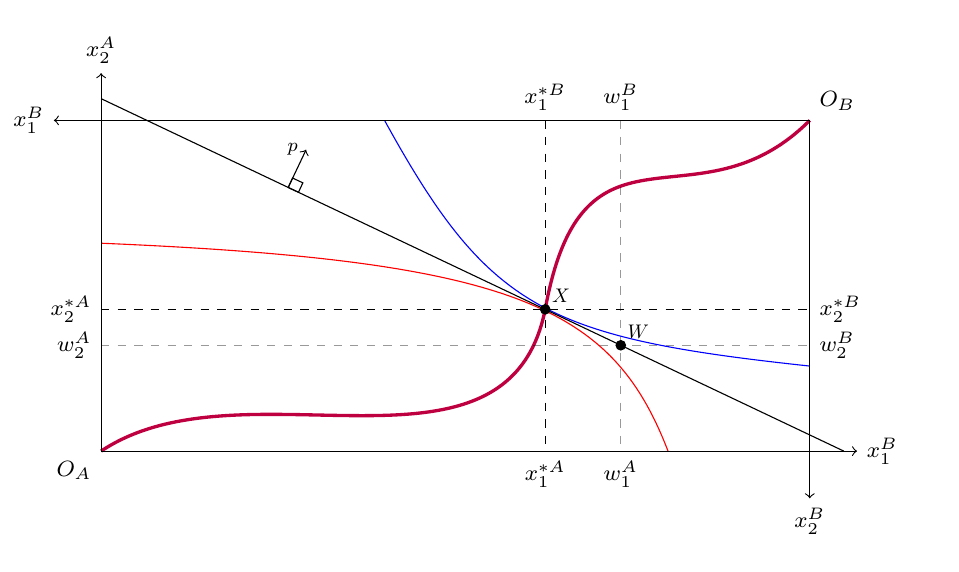
\begin{tikzpicture}[scale=1.2]
	\hspace{-0.3cm}
	% Curva de contrato 5.2,2
		\draw  [purple, very thick] (0.5,0.5) ..controls (2,1.5) and (4.8,0) .. (5.2,2) ..controls (5.6,4.2) and (6.8,2.8) .. (8,4);
	% Intersección de una dotación
		% Demanda: x
			\draw[dashed] (5.2,4) node[above] {\footnotesize $x_{1}^{*B}$} -- (5.2,0.5) node[below]{\footnotesize $x_{1}^{*A}$};
			\draw[dashed] (0.5,2) node[left] {\footnotesize $x_{2}^{*A}$} -- (8,2)node[right]{\footnotesize $x_{2}^{*B}$};
		
		% Oferta: w
			\draw[dashed, opacity=0.4] (6,4) -- (6,0.5);
			\draw[dashed, opacity=0.4] (0.5,1.62)  -- (8,1.62);
			
			\draw (8,1.62)  node [right] {\footnotesize $w_{2}^{B}$};
			\draw (6,4)  node [above] {\footnotesize $w_{1}^{B}$};
			
			\draw (0.5,1.62)  node [left] {\footnotesize $w_{2}^{A}$};
			\draw (6,0.5)  node [below] {\footnotesize $w_{1}^{A}$};
	
	% Curvas de indiferencia
		\draw [blue] (3.5,4) .. controls (4.6,2) and (5.2,1.7) .. (8,1.4);
		\draw [red] (0.5,2.7) .. controls (4.915,2.515) and (5.915,2.015) .. (6.5,0.5);
	
	% Recta presupuestaria
		\draw (0.5,4.23) -- (8.36,0.5);
	
	% Puntos
		\draw[black, fill=black] (5.2,2) circle[radius=0.05] node [above right, scale=0.25mm] {$X$};
		\draw[black, fill=black] (6,1.62) circle[radius=0.05] node [above right, scale=0.25mm] {$W$};
	
	% Flecha y rectángulo
		\draw [->] (2.48,3.29) -- (2.67,3.69) node [left, scale = 0.3mm] {\footnotesize $p$};
		\draw [rotate around={-25:(2.48,3.29)}] (2.48,3.29) rectangle (2.6, 3.4);
		
	% Formación de la caja
		% Consumidor A
			\draw[->] (0.5,0.5) node[align=center, below left] {\footnotesize $O_A$} -- (0.5,4.5) node[align=center, above] {\footnotesize $x_{2}^{A}$};
			\draw[->] (0.5,0.5) -- (8.5,0.5) node[align=center, right] {\footnotesize $x_{1}^{B}$};
		
		%Consumidor B
			\draw[->] (8,4) node[align=center, above right] {\footnotesize $O_B$} -- (0,4) node[align=center, left] {\footnotesize $x_{1}^{B}$};
			\draw[->] (8,4) -- (8,0) node[align=center, below] {\footnotesize $x_{2}^{B}$};
\end{tikzpicture}
		\end{center}
	\end{multicols}
\end{frame}
%------------------------------------------------
\begin{frame}{Externalidades de consumo}
	\begin{center}
		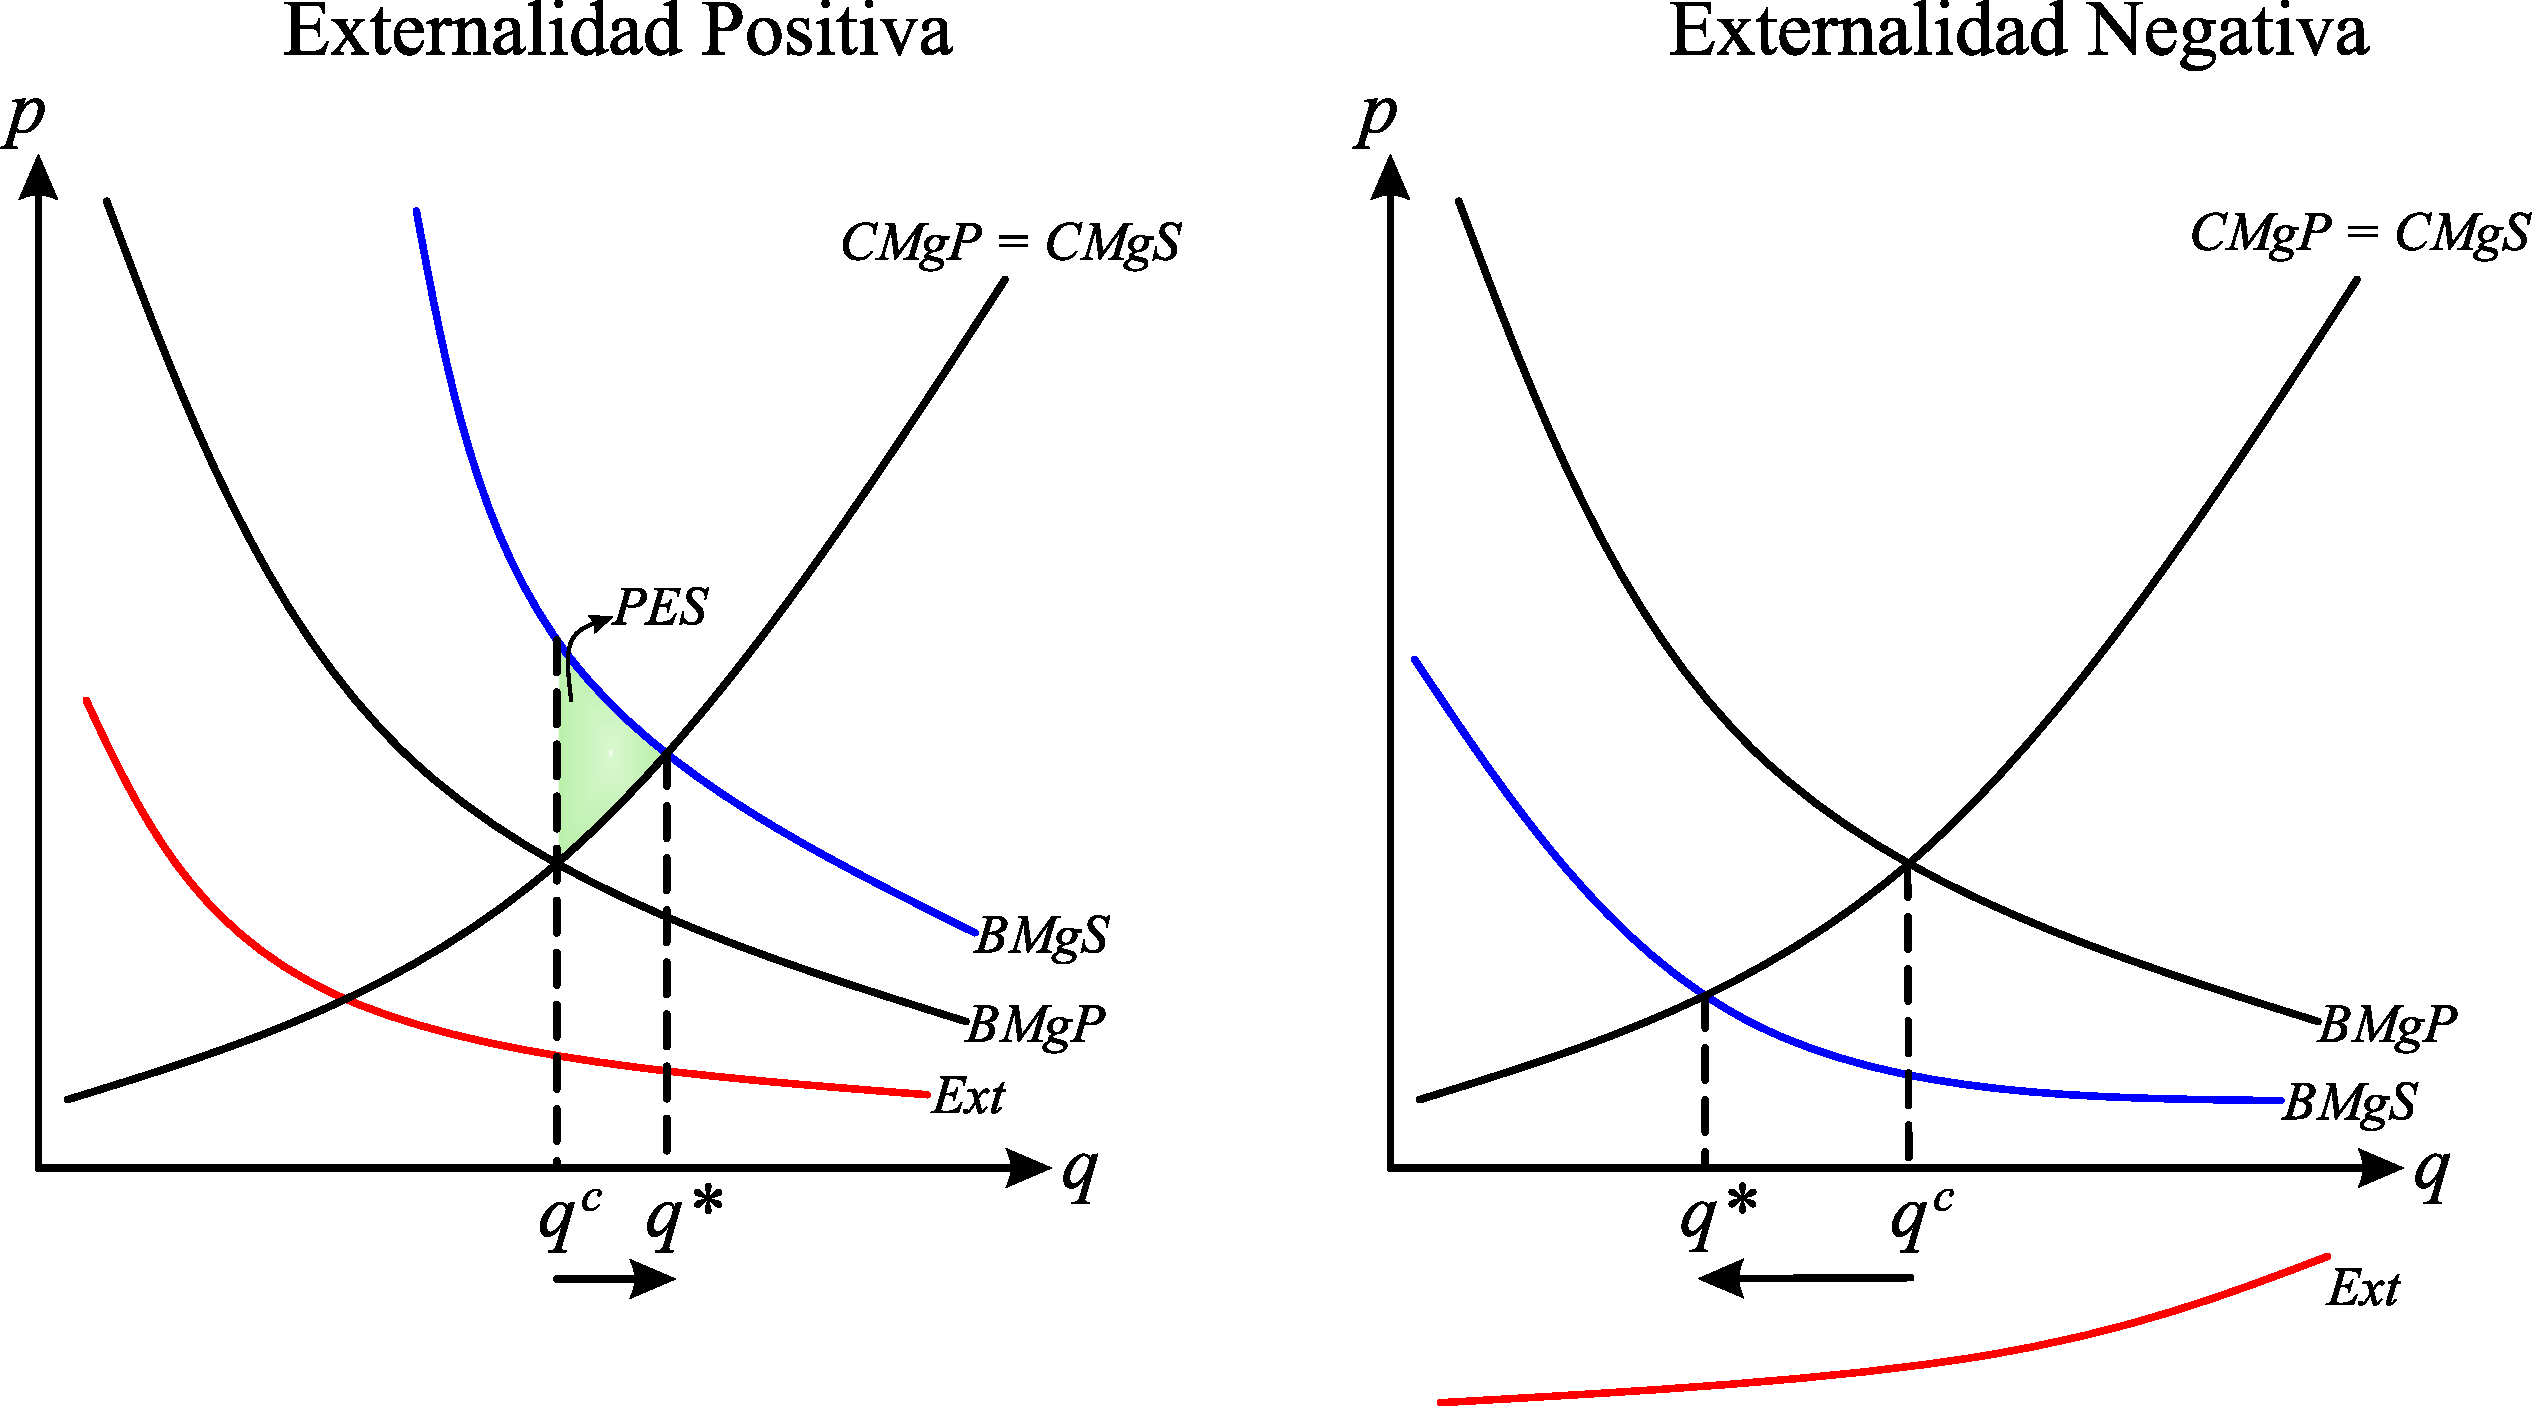
\includegraphics[width = 1\linewidth]{figures/consumo.pdf}
	\end{center}
\end{frame}